%Copyright (c) 2004 2005 2006 Atos Origin
%Permission is granted to copy, distribute and/or modify this
%document
%under the terms of the GNU Free Documentation License,
%      Version 1.2
%      or any later version published by the Free Software
%      Foundation;
%      with no Invariant Sections, no Front-Cover
%      Texts, and no Back-Cover
%      Texts.  A copy of the license is
%      included in the section entitled "GNU
%      Free Documentation License".
%
%$Id: select.tex,v 1.1 2006/02/16 16:33:33 goneri Exp $
\section{Select}
\begin{figure}[h]
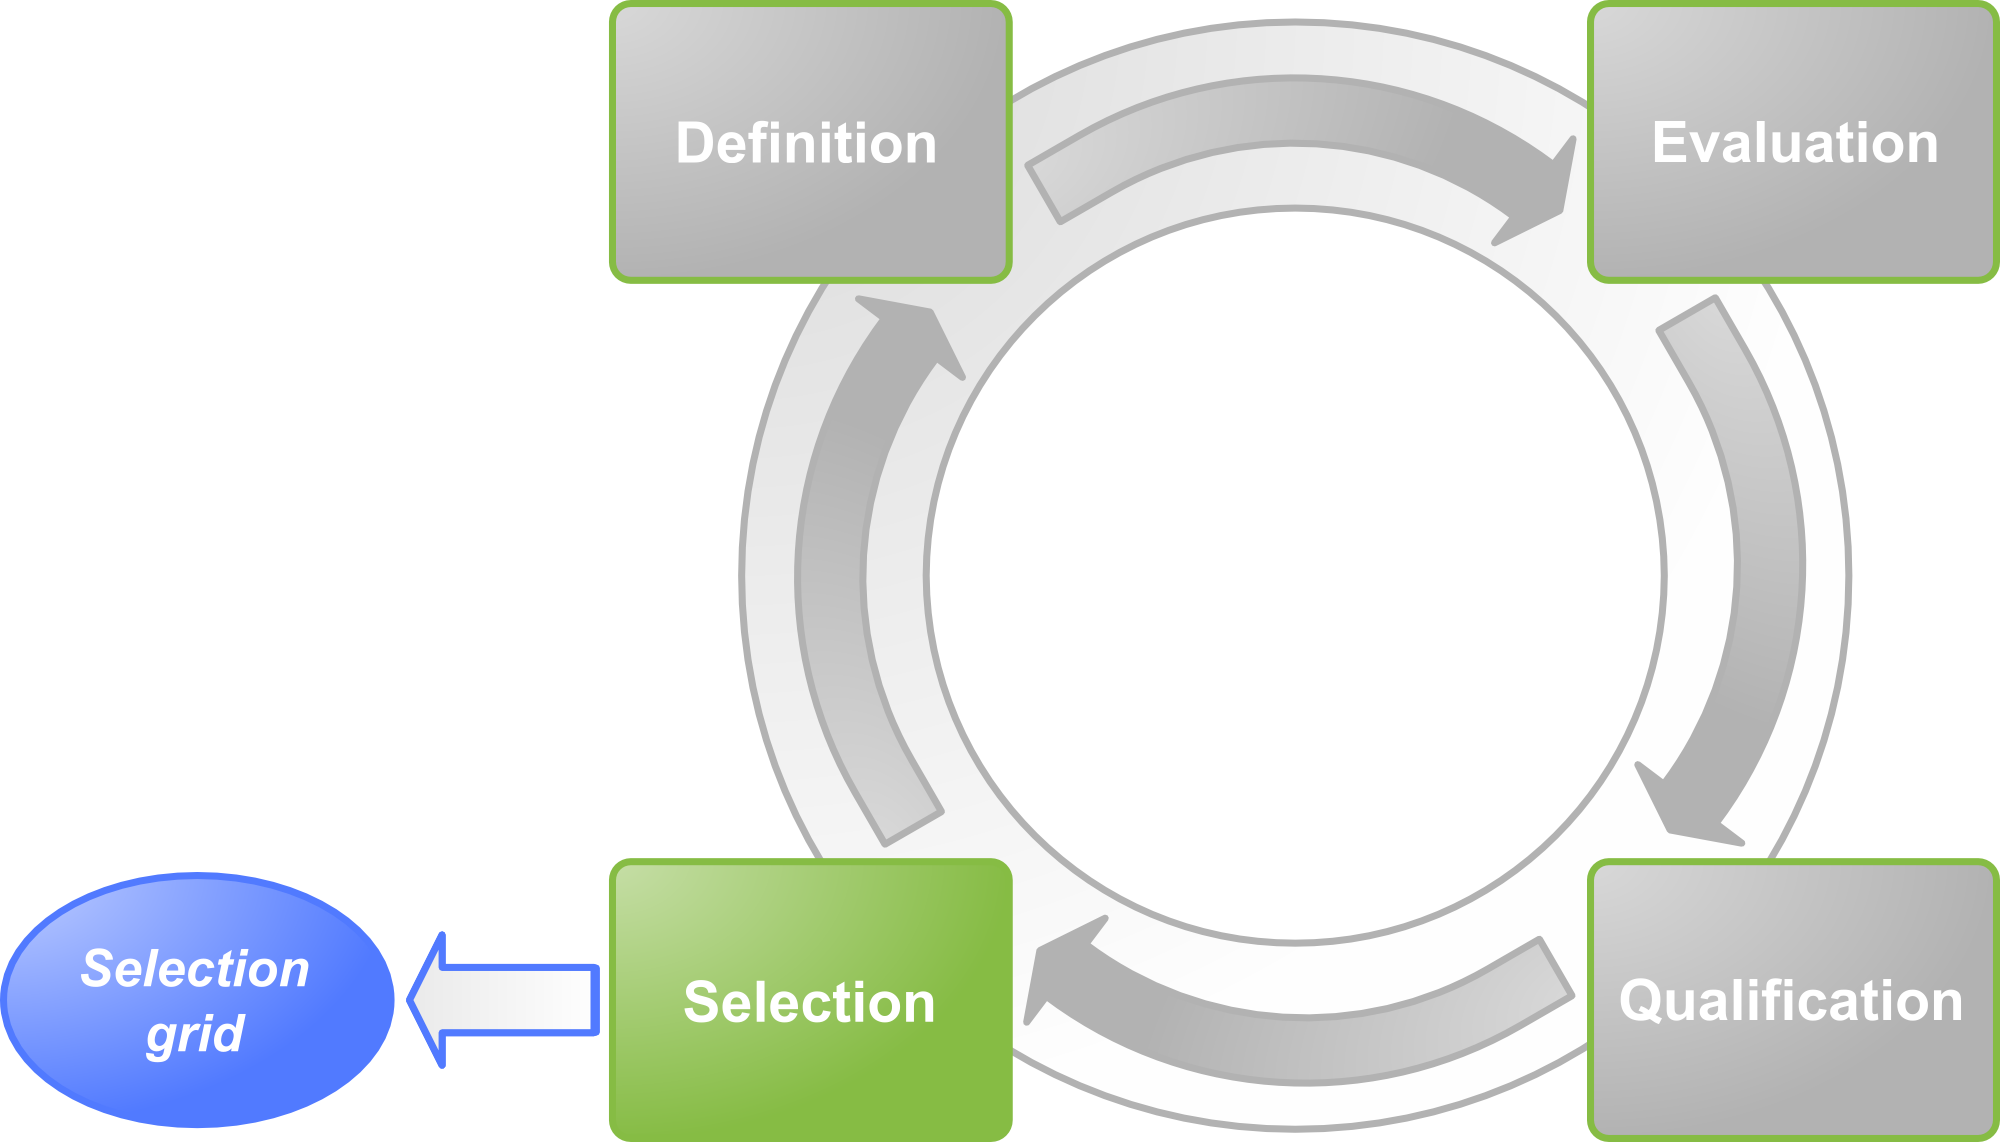
\includegraphics[width=13cm]{images/selectionner}
\caption{Step 4 - Select}
\end{figure}

\subsection{Objective}
The objective of this step is to identify software fulfilling user's requirements, 
or more generally to compare software from the same family.

\subsection{Selection}
Two modes are possible:
\begin{itemize}
\item strict selection
\item loose selection
\end{itemize}


\subsubsection{Strict selection}
Strict selection is based on direct elimination as soon as a software
does does not fulfill the requirements formulated in Step 3 - "Qualify":

\begin{itemize}
\item Elimination of software incompatible with the filter on ID card
\item Elimination of software not providing functionality required by the filter on the functional grid
\item Elimination of software whose scores on the user's risks axis do not meet the relevance defined by or with the user:
\begin{itemize}
\item The score of a relevant criterion must be at least equal to 1
\item The score of a critical criterion must be at least equal to 2
\end{itemize}
\end{itemize}
This method is very selective and may, depending on user's requirement, return no eligible software.


Selected software are then attributed a total score, calculated by weighting as for loose selection.

\subsubsection{Loose selection}
This method is less strict than the previous because rather than to eliminate non-eligible software, it classifies them while measuring the gaps with applied filters.

The rules of weighting to use are detailed in following paragraphs.


\paragraph{Weighting of functionalities}
The weighting value is based on the level of requirement defined on each functionality of the functional grid.
\begin{figure}
\center
\begin{tabular}{|c|c|}
\hline \TS{Level of requirement} & \TS{Weight}\\
\hline Required functionality & +3\\
\hline Optional functionality & +1\\
\hline Not required functionality & 0\\
\hline
\end{tabular}
\end{figure}

\paragraph{Weighting on User's risk axis}
The weighting value is based on the relevance of each criterion on the user's risk axis.
\begin{figure}
\center
\begin{tabular}{|c|c|}
\hline \TS{Relevance} & \TS{Weight}\\
\hline Irrelevant criterion & 0\\
\hline Relevant criterion & +1 or -1\\
\hline Critical criterion & +3 or -3\\
\hline
\end{tabular}
\end{figure}

The weight's value sign represents a positive or negative impact regarding the user's requirements.

\subsection{Comparison}
The software of a same family (with a common functionnal grid) can also be compared by using weighted scores determined earlier.


Figure~\ref{fig-comparaison} illustrates the kind of synthesis available.
\begin{figure}
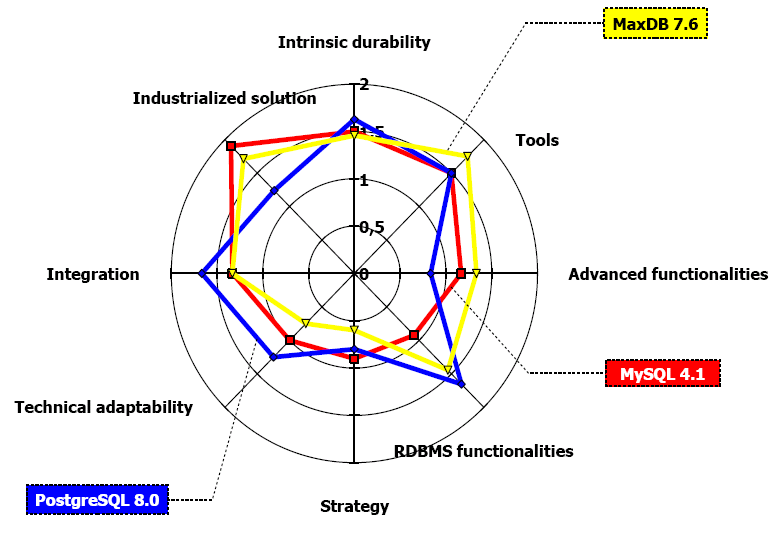
\includegraphics[height=10cm]{images/comparaison}
\caption{
Comparison. 
This figure is provided as an example, therefore weightings on the various axis are not representative of all kind of RDMBS utilisations.
}
\label{fig-comparaison}
\end{figure}

\subsection{O3S tool}
Besides implementing the strict and loose selection modes, the O3S tool also allows to consult data related to a specific software (ID card and evaluation criteria) and to compare (integrally, by filtering or differentially) software of a same family.